\documentclass[border=10pt]{standalone}
\usepackage[svgnames]{xcolor}
\usepackage{amsmath}
\usepackage{pgfplots}
\pgfplotsset{compat=newest}
\usepackage[sfdefault]{FiraSans}
\usepackage{FiraMono}
\renewcommand*\familydefault{\sfdefault}
\begin{document}
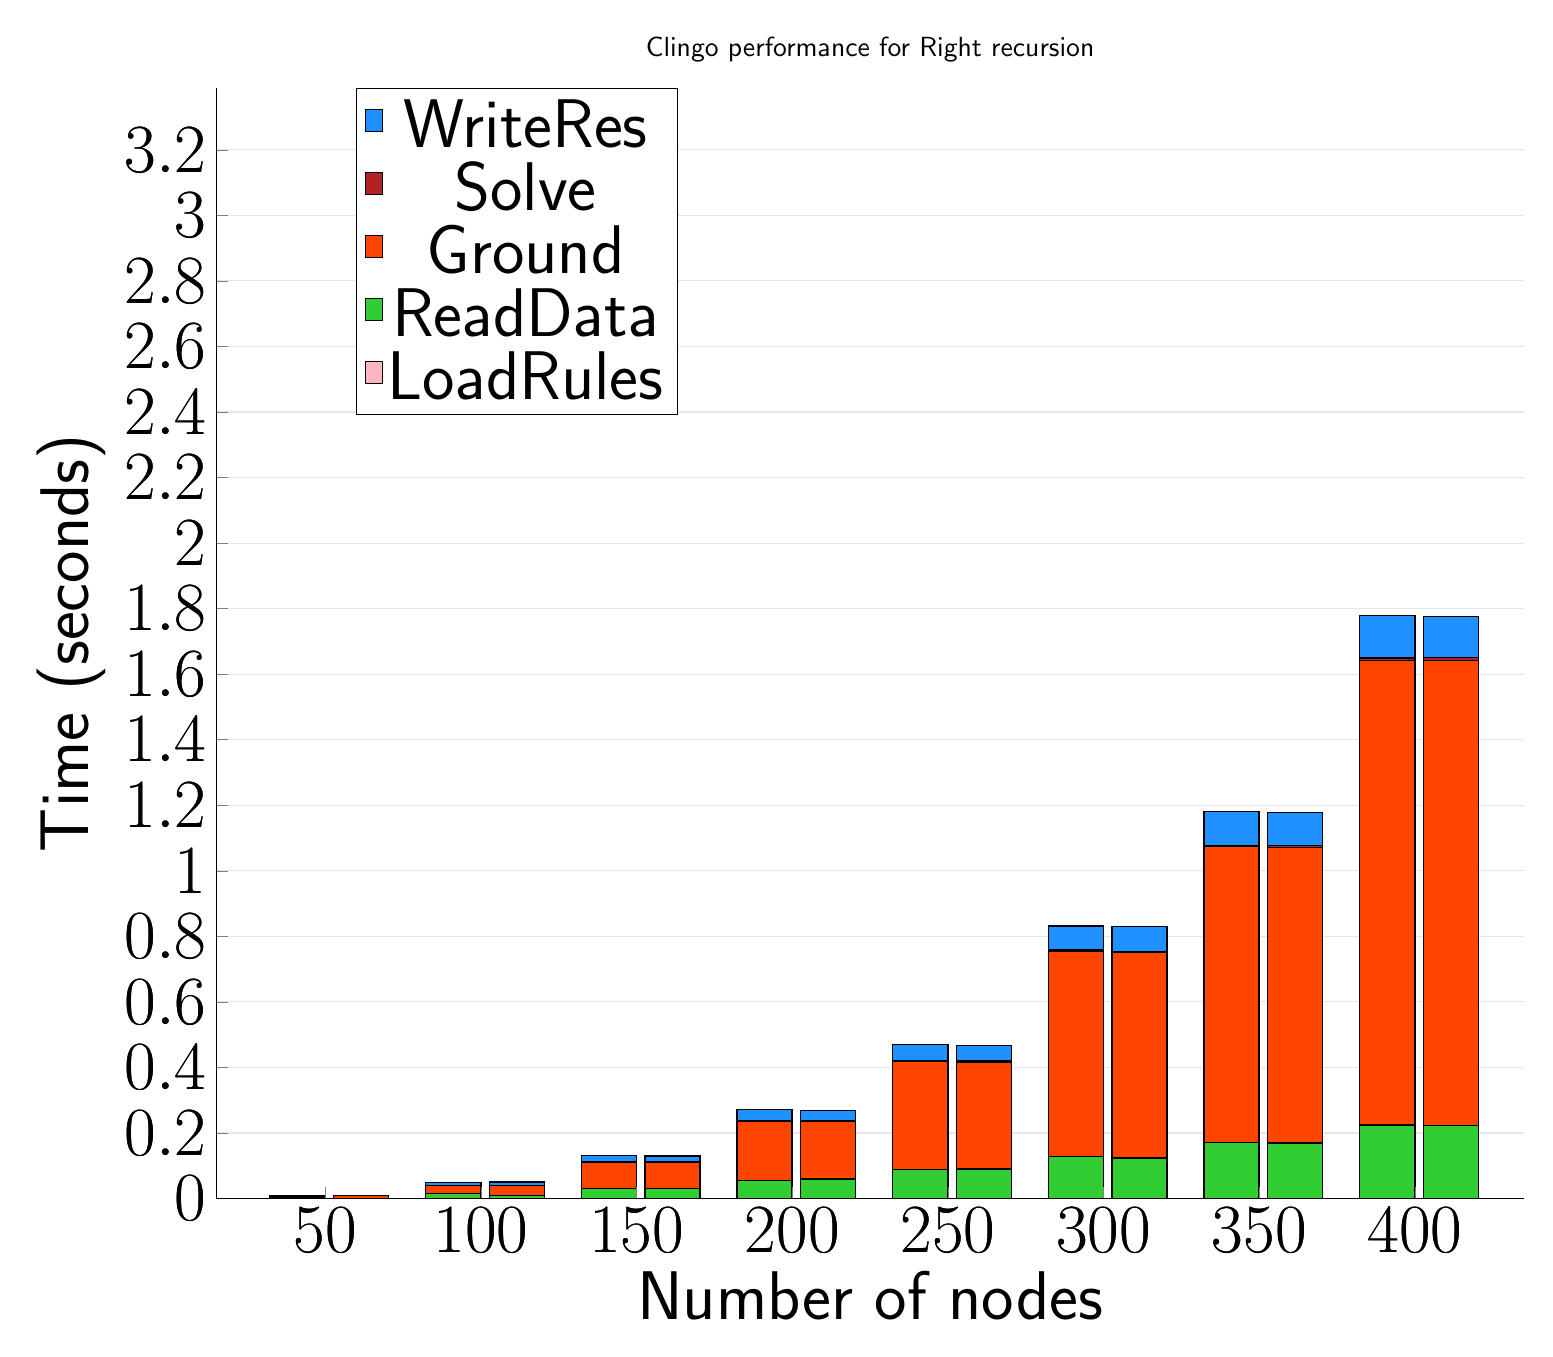
\begin{tikzpicture}
	\begin{axis}[
			ybar stacked,
			title={Clingo performance for Right recursion},
			bar shift=-10pt,
			width=1.5\textwidth,
			bar width=0.7cm,
			ymajorgrids, tick align=inside,
			major grid style={draw=gray!20},
			xtick=data,
			ymin=0, ymax=3.3890000581741333,
			axis x line*=bottom,
			axis y line*=left,
			enlarge x limits=0.1,
			legend style={
					at={(0.23, 1)},
					anchor=north,
					legend columns=1,
					font=\Huge,
				},
			ylabel={Time (seconds)},
			xlabel={Number of nodes},
			label style={font=\Huge},
			tick label style={font=\Huge},
		]
		\addlegendimage{fill=DodgerBlue, draw=black, line width=0.2pt}
		\addlegendentry{WriteRes}
		\addlegendimage{fill=FireBrick, draw=black, line width=0.2pt}
		\addlegendentry{Solve}
		\addlegendimage{fill=OrangeRed, draw=black, line width=0.2pt}
		\addlegendentry{Ground}
		\addlegendimage{fill=LimeGreen, draw=black, line width=0.2pt}
		\addlegendentry{ReadData}
		\addlegendimage{fill=LightPink, draw=black, line width=0.2pt}
		\addlegendentry{LoadRules}
		\addplot +[fill=LightPink, draw=black, line width=0.5pt] coordinates {
				(50, 0.0)
				(100, 0.0)
				(150, 0.0)
				(200, 0.0)
				(250, 0.0)
				(300, 0.0)
				(350, 0.0)
				(400, 0.0)
			};
		\addplot +[fill=LimeGreen, draw=black, line width=0.5pt] coordinates {
				(50, 0.0039999961853027345)
				(100, 0.015000009536743164)
				(150, 0.029999971389770508)
				(200, 0.05499999523162842)
				(250, 0.08799993991851807)
				(300, 0.12799999713897706)
				(350, 0.17100002765655517)
				(400, 0.2250000238418579)
			};
		\addplot +[fill=OrangeRed, draw=black, line width=0.5pt] coordinates {
				(50, 0.003000020980834961)
				(100, 0.023999977111816406)
				(150, 0.0820000171661377)
				(200, 0.1809999942779541)
				(250, 0.3299999713897705)
				(300, 0.6269999980926514)
				(350, 0.9040000677108765)
				(400, 1.4169999837875367)
			};
		\addplot +[fill=FireBrick, draw=black, line width=0.5pt] coordinates {
				(50, 0.0)
				(100, 0.0009999990463256836)
				(150, 0.0009999990463256836)
				(200, 0.0009999990463256836)
				(250, 0.0029999971389770507)
				(300, 0.0029999971389770507)
				(350, 0.0029999971389770507)
				(400, 0.006999993324279785)
			};
		\addplot +[fill=DodgerBlue, draw=black, line width=0.5pt] coordinates {
				(50, 0.0019999980926513673)
				(100, 0.008999991416931152)
				(150, 0.017999982833862303)
				(200, 0.03400001525878906)
				(250, 0.05000004768371582)
				(300, 0.07400004863739014)
				(350, 0.10299992561340332)
				(400, 0.13000001907348632)
			};
	\end{axis}
	\begin{axis}[
			ybar stacked,
			bar shift=13pt,
			width=1.5\textwidth,
			bar width=0.7cm,
			ymajorgrids, tick align=inside,
			major grid style={draw=none},
			xtick=data,
			ymin=0, ymax=3.3890000581741333,
			axis x line*=none,
			axis y line*=none,
			enlarge x limits=0.1,
			label style={font=\Huge},
			tick label style={font=\Huge},
		]
		\addplot +[fill=LightPink, draw=black, line width=0.5pt] coordinates {
				(50, 0.0)
				(100, 0.0)
				(150, 0.0)
				(200, 0.0)
				(250, 0.0)
				(300, 0.0)
				(350, 0.0)
				(400, 0.0)
			};
		\addplot +[fill=LimeGreen, draw=black, line width=0.5pt] coordinates {
				(50, 0.0)
				(100, 0.009999999999999997)
				(150, 0.030000000000000006)
				(200, 0.06000000000000001)
				(250, 0.08999999999999998)
				(300, 0.12400000000000003)
				(350, 0.16999999999999998)
				(400, 0.22300000000000003)
			};
		\addplot +[fill=OrangeRed, draw=black, line width=0.5pt] coordinates {
				(50, 0.009999999999999997)
				(100, 0.030000000000000006)
				(150, 0.08199999999999999)
				(200, 0.17499999999999996)
				(250, 0.326)
				(300, 0.6279999999999999)
				(350, 0.9010000000000001)
				(400, 1.418)
			};
		\addplot +[fill=FireBrick, draw=black, line width=0.5pt] coordinates {
				(50, 0.0)
				(100, 0.0)
				(150, 0.0010000000000000009)
				(200, 0.0030000000000000027)
				(250, 0.0040000000000000036)
				(300, 0.0020000000000000018)
				(350, 0.007000000000000006)
				(400, 0.010000000000000009)
			};
		\addplot +[fill=DodgerBlue, draw=black, line width=0.5pt] coordinates {
				(50, 0.0)
				(100, 0.010000000000000009)
				(150, 0.016999999999999994)
				(200, 0.03099999999999999)
				(250, 0.046999999999999986)
				(300, 0.07599999999999997)
				(350, 0.09999999999999987)
				(400, 0.12500000000000006)
			};
	\end{axis}
\end{tikzpicture}

\end{document}
